\documentclass[article, 12pt, oneside, a4paper, section = TITLE, brazil]{abntex2}

\usepackage{times}
\usepackage[T1]{fontenc}	
\usepackage[utf8]{inputenc}		
\usepackage{indentfirst}		
\usepackage{color}				
\usepackage{graphicx}			
\usepackage{microtype} 		
\usepackage{multirow}
\usepackage{lscape}
\usepackage{amsmath}
\usepackage{breqn} 
\usepackage{hhline}
\usepackage{caption}
\usepackage[table,xcdraw]{xcolor}
\usepackage{mathptmx}
\usepackage{float}
\usepackage{xcolor}
\usepackage{float}
\usepackage{graphicx}
\usepackage{multirow}
\usepackage{lipsum}
\usepackage{textcomp}
\usepackage[num]{abntex2cite}
\usepackage{longtable} 
\usepackage{booktabs} 
\usepackage{listings}
\usepackage{xcolor}
\usepackage{array}

\lstset{
    language=Python,
    basicstyle=\ttfamily\small,
    breaklines=true,
    frame=single,
    columns=fullflexible,
    keepspaces=true,
    showstringspaces=false
}

\renewcommand{\ABNTEXchapterfont}{\rmfamily}
\renewcommand{\ABNTEXsectionfont}{\rmfamily}
\renewcommand{\ABNTEXsubsectionfont}{\rmfamily}

\makeatletter\@removefromreset{equation}{section}\makeatother	

\ABNTEXfontereduzida 
\renewcommand{\ABNTEXchapterfontsize}{\normalsize}
\renewcommand{\ABNTEXsectionfontsize}{\normalsize}
\renewcommand{\ABNTEXsubsectionfontsize}{\normalsize}

\setlrmarginsandblock{3cm}{2cm}{*}
\setulmarginsandblock{3cm}{2cm}{*}
\checkandfixthelayout

\setlength{\parindent}{1.3cm}

\setlength{\parskip}{0.2cm} 


\makeatletter
\let\@fnsymbol\@arabic
\makeatother	

\makeatletter

\def\@maketitle{	
	\begin{center}
 \textbf{OPTATIVA III REDES NEURAIS ARTIFICIAIS - 7\textsuperscript{o} PERÍODO - ENG. COMP} \\
Universidade do Estado de Minas Gerais - UEMG
\vskip 2em
    {\Large \@title  \par \textbf{\textit{\imprimirtituloestrangeiro}} }
		\vskip 3em
		{\normalsize \flushright
			\lineskip .5em
			\begin{tabular}[t]{c}
				\@author
			\end{tabular}\par}
		\vskip 1em
 \eixo
	\end{center}
	\vskip 1.5em}
\makeatother






\titulo{\textbf{5\textsuperscript{o} Projeto Prático – Rede RBF no Reconhecimento de Padrões}}

\autor{
    ÍTALO VINÍCIUS DE BESSA - 1699833\thanks{Universidade do Estado de Minas Gerais - UEMG. italo.1699833@discente.uemg.br}
    \\[0.2cm]
    YAN GABRIEL FERREIRA DA CRUZ - 1699690\thanks{Universidade do Estado de Minas Gerais - UEMG. yan.1699690@discente.uemg.br}
}

\newcommand{\eixo}{}

\lstset{literate={θ}{{\ensuremath{\theta}}}{1}}

\begin{document}
\pagestyle{plain}
\maketitle
\frenchspacing
\selectlanguage{brazil}

\clearpage

% =============================================================
\section*{1. Código utilizado}
% =============================================================

A implementação foi realizada em um único arquivo (\texttt{rbf.py}), contemplando a preparação dos dados, o treinamento em dois estágios (K-Means e Regra Delta), a validação e a geração de gráficos e planilhas.

\begin{lstlisting}
import os
import math
import numpy as np
import pandas as pd
import matplotlib.pyplot as plt

DADOS_TREINAMENTO = np.array([
    [0.2563, 0.9503, -1], [0.2405, 0.9018, -1], [0.1157, 0.3676,  1],
    [0.5147, 0.0167,  1], [0.4127, 0.3275,  1], [0.2809, 0.5830,  1],
    [0.8263, 0.9301, -1], [0.9359, 0.8724, -1], [0.1096, 0.9165, -1],
    [0.5158, 0.8545, -1], [0.1334, 0.1362,  1], [0.6371, 0.1439,  1],
    [0.7052, 0.6277, -1], [0.8703, 0.8666, -1], [0.2612, 0.6109,  1],
    [0.0244, 0.5279,  1], [0.9588, 0.3672, -1], [0.9332, 0.5499, -1],
    [0.9623, 0.2961, -1], [0.7297, 0.5776, -1], [0.4560, 0.1871,  1],
    [0.1715, 0.7713,  1], [0.5571, 0.5485, -1], [0.3344, 0.0259,  1],
    [0.4803, 0.7635, -1], [0.9721, 0.4850, -1], [0.8318, 0.7844, -1],
    [0.1373, 0.0292,  1], [0.3660, 0.8581, -1], [0.3626, 0.7302, -1],
    [0.6474, 0.3324,  1], [0.3461, 0.2398,  1], [0.1353, 0.8120,  1],
    [0.3463, 0.1017,  1], [0.9086, 0.1947, -1], [0.5227, 0.2321,  1],
    [0.5153, 0.2041,  1], [0.1832, 0.0661,  1], [0.5015, 0.9812, -1],
    [0.5024, 0.5274, -1],
])

DADOS_VALIDACAO = np.array([
    [0.8705, 0.9329, -1], [0.0388, 0.2703,  1], [0.8236, 0.4458, -1],
    [0.7075, 0.1502,  1], [0.9587, 0.8663, -1], [0.6115, 0.9365, -1],
    [0.3534, 0.3646,  1], [0.3268, 0.2766,  1], [0.6129, 0.4518, -1],
    [0.9948, 0.4962, -1],
])

ETA        = 0.01
EPSILON    = 1e-7
MAX_EPOCAS = 100_000
K          = 2
N_REDES    = 5

DATASETS_PATH           = os.path.join(os.getcwd(), 'datasets')
EVOLUCAO_PATH           = os.path.join(os.getcwd(), 'graphics', 'Evolucao_do_erro')
MATRIZES_PATH           = os.path.join(os.getcwd(), 'graphics', 'matrizes_de_confusao')
GRAFICOS_VALIDACAO_PATH = os.path.join(os.getcwd(), 'graphics', 'validacao')


def preparar_datasets():
    os.makedirs(DATASETS_PATH, exist_ok=True)
    df_treino = pd.DataFrame(DADOS_TREINAMENTO, columns=['x1', 'x2', 'd'])
    df_treino['d'] = df_treino['d'].astype(int)
    df_treino.to_excel(os.path.join(DATASETS_PATH, 'rbf_treinamento.xlsx'), index=False)
    df_val = pd.DataFrame(DADOS_VALIDACAO, columns=['x1', 'x2', 'd'])
    df_val['d'] = df_val['d'].astype(int)
    df_val.to_excel(os.path.join(DATASETS_PATH, 'rbf_validacao.xlsx'), index=False)
    print("  Datasets preparados em datasets/")


def carregar_dados():
    df_treino = pd.read_excel(os.path.join(DATASETS_PATH, 'rbf_treinamento.xlsx'))
    df_val    = pd.read_excel(os.path.join(DATASETS_PATH, 'rbf_validacao.xlsx'))
    X_treino = df_treino[['x1', 'x2']].values
    D_treino = df_treino['d'].values.astype(float)
    X_val    = df_val[['x1', 'x2']].values
    D_val    = df_val['d'].values.astype(float)
    return X_treino, D_treino, X_val, D_val


def salvar_validacao(X_val, D_val, predicoes_cont, predicoes_bin):
    df = pd.DataFrame({'x1': X_val[:, 0], 'x2': X_val[:, 1],
                       'd':  [int(d) for d in D_val]})
    for T in range(1, N_REDES + 1):
        df[f'y_T{T}']    = [round(v, 8) for v in predicoes_cont[T]]
        df[f'ybin_T{T}'] = predicoes_bin[T]
    df.to_excel(os.path.join(DATASETS_PATH, 'rbf_validacao.xlsx'), index=False)
    print("  Previsoes salvas em datasets/rbf_validacao.xlsx")


def salvar_metricas(resultados):
    linhas = []
    for r in resultados:
        linhas.append({
            'Rede':               f"T{r['T']}",
            'Epocas':             r['epocas'],
            'EQM Final':          round(r['eqm_final'], 8),
            'VP':                 r['VP'],
            'VN':                 r['VN'],
            'FP':                 r['FP'],
            'FN':                 r['FN'],
            'Acertos':            r['acertos'],
            'Erros':              r['erros'],
            'Acuracia (%)':       round(r['acuracia']       * 100, 2),
            'Sensibilidade (%)':  round(r['sensibilidade']  * 100, 2),
            'Especificidade (%)': round(r['especificidade'] * 100, 2),
            'Precisao (%)':       round(r['precisao']       * 100, 2),
        })
    pd.DataFrame(linhas).to_excel(
        os.path.join(DATASETS_PATH, 'rbf_metricas.xlsx'), index=False)
    print("  Metricas salvas em datasets/rbf_metricas.xlsx")


def salvar_treinamentos(treinamentos):
    linhas = []
    for t in treinamentos:
        linhas.append({
            'Rede':                  f"T{t['T']}",
            'Cluster 1 - Centro x1': round(float(t['c1'][0]), 8),
            'Cluster 1 - Centro x2': round(float(t['c1'][1]), 8),
            'Cluster 1 - Variancia': round(float(t['v1']), 8),
            'Cluster 2 - Centro x1': round(float(t['c2'][0]), 8),
            'Cluster 2 - Centro x2': round(float(t['c2'][1]), 8),
            'Cluster 2 - Variancia': round(float(t['v2']), 8),
            'W1 (W11^(2))':          round(float(t['W'][0]), 8),
            'W2 (W21^(2))':          round(float(t['W'][1]), 8),
            'theta':                 round(float(t['theta']), 8),
            'Epocas':                t['epocas'],
            'EQM Final':             round(float(t['eqm_final']), 8),
        })
    pd.DataFrame(linhas).to_excel(
        os.path.join(DATASETS_PATH, 'rbf_treinamentos.xlsx'), index=False)
    print("  Parametros de treinamento salvos em datasets/rbf_treinamentos.xlsx")


def gaussiana(x, centro, sigma2):
    dist2    = float(np.sum((x - centro) ** 2))
    expoente = -dist2 / (2.0 * sigma2)
    return math.exp(max(expoente, -500.0))


def calcular_phi(x, centros, variancias):
    return np.array([gaussiana(x, centros[i], variancias[i]) for i in range(K)])


def propagacao_direta(x, centros, variancias, W, theta):
    phi = calcular_phi(x, centros, variancias)
    y   = float(np.dot(W, phi)) + theta
    return phi, y


def pos_processar(y):
    return 1 if y >= 0.0 else -1


def kmeans(X_pos, k=K, max_iter=1000):
    n        = len(X_pos)
    idx_init = np.random.choice(n, k, replace=False)
    centros  = X_pos[idx_init].copy().astype(float)
    for _ in range(max_iter):
        dists   = np.array([[np.sum((x - c) ** 2) for c in centros]
                             for x in X_pos])
        rotulos = np.argmin(dists, axis=1)
        novos_centros = np.zeros_like(centros)
        for i in range(k):
            membros = X_pos[rotulos == i]
            novos_centros[i] = (membros.mean(axis=0) if len(membros) > 0
                                else X_pos[np.random.randint(n)])
        if np.allclose(centros, novos_centros, atol=1e-12):
            break
        centros = novos_centros
    return centros, rotulos


def calcular_variancias(X_pos, centros, rotulos, k=K):
    variancias = []
    for i in range(k):
        membros = X_pos[rotulos == i]
        if len(membros) > 1:
            var = float(2.0 * np.mean(np.sum((membros - centros[i]) ** 2, axis=1)))
        else:
            var = 1e-6
        variancias.append(max(var, 1e-12))
    return np.array(variancias)


def treinar_saida(X_treino, D_treino, centros, variancias):
    W     = np.random.uniform(-0.1, 0.1, K)
    theta = float(np.random.uniform(-0.1, 0.1))
    eqm_por_epoca = []
    eqm_anterior  = float('inf')
    for epoca in range(MAX_EPOCAS):
        erros_quad = []
        for x, d in zip(X_treino, D_treino):
            phi, y = propagacao_direta(x, centros, variancias, W, theta)
            e      = d - y
            erros_quad.append(e ** 2)
            W     += ETA * e * phi
            theta += ETA * e
        eqm = float(0.5 * np.mean(erros_quad))
        eqm_por_epoca.append(eqm)
        if abs(eqm_anterior - eqm) < EPSILON:
            print(f"  Convergencia na epoca {epoca + 1}  |  EQM = {eqm:.2e}")
            break
        eqm_anterior = eqm
    else:
        print(f"  Limite de {MAX_EPOCAS} epocas  |  EQM = {eqm_por_epoca[-1]:.2e}")
    return W, theta, eqm_por_epoca


def calcular_metricas(y_pred, y_real):
    VP = sum(1 for p, r in zip(y_pred, y_real) if p ==  1 and r ==  1)
    VN = sum(1 for p, r in zip(y_pred, y_real) if p == -1 and r == -1)
    FP = sum(1 for p, r in zip(y_pred, y_real) if p ==  1 and r == -1)
    FN = sum(1 for p, r in zip(y_pred, y_real) if p == -1 and r ==  1)
    total   = len(y_pred)
    acertos = VP + VN
    erros   = FP + FN
    return {
        'VP': VP, 'VN': VN, 'FP': FP, 'FN': FN,
        'acertos': acertos, 'erros': erros,
        'acuracia':       acertos / total,
        'sensibilidade':  VP / (VP + FN) if (VP + FN) > 0 else 0.0,
        'especificidade': VN / (VN + FP) if (VN + FP) > 0 else 0.0,
        'precisao':       VP / (VP + FP) if (VP + FP) > 0 else 0.0,
    }


def plotar_eqm(eqm_por_epoca, T):
    os.makedirs(EVOLUCAO_PATH, exist_ok=True)
    epocas = list(range(1, len(eqm_por_epoca) + 1))
    fig, ax = plt.subplots(figsize=(10, 5))
    ax.plot(epocas, eqm_por_epoca, linewidth=1.2, color='steelblue')
    ax.set_title(f'Evolucao do EQM - Rede RBF T{T} (Regra Delta)')
    ax.set_xlabel('Epocas')
    ax.set_ylabel('Erro Quadratico Medio (EQM)')
    ax.grid(True, alpha=0.4)
    fig.tight_layout()
    caminho = os.path.join(EVOLUCAO_PATH, f'treinamento_rbf_{T}.png')
    fig.savefig(caminho, dpi=150)
    plt.close(fig)
    print(f"  Grafico EQM salvo em: {caminho}")


def plotar_validacao(X_val, D_val, y_cont, T):
    os.makedirs(GRAFICOS_VALIDACAO_PATH, exist_ok=True)
    amostras = list(range(1, len(X_val) + 1))
    fig, ax = plt.subplots(figsize=(10, 5))
    ax.plot(amostras, D_val, 'b-o', label='Saida desejada (d)',
            markersize=5, linewidth=1.5)
    ax.plot(amostras, y_cont, 'r-s', label=f'Saida da rede T{T} (y)',
            markersize=5, linewidth=1.5)
    ax.set_title(f'Validacao T{T}: Saida Desejada vs. Saida da Rede RBF')
    ax.set_xlabel('Numero da amostra')
    ax.set_ylabel('Saida')
    ax.legend()
    ax.grid(True, alpha=0.4)
    ax.set_xticks(amostras)
    fig.tight_layout()
    caminho = os.path.join(GRAFICOS_VALIDACAO_PATH, f'validacao_rbf_T{T}.png')
    fig.savefig(caminho, dpi=150)
    plt.close(fig)
    print(f"  Grafico de validacao salvo em: {caminho}")


def plotar_matriz_confusao(m, T):
    os.makedirs(MATRIZES_PATH, exist_ok=True)
    matriz = np.array([[m['VP'], m['FN']], [m['FP'], m['VN']]])
    fig, ax = plt.subplots(figsize=(5, 4))
    im = ax.imshow(matriz, cmap='Blues', vmin=0)
    ax.set_xticks([0, 1])
    ax.set_yticks([0, 1])
    ax.set_xticklabels(['+1\n(Previsto)', '-1\n(Previsto)'], fontsize=10)
    ax.set_yticklabels(['+1 (Real)', '-1 (Real)'], fontsize=10)
    for i in range(2):
        for j in range(2):
            ax.text(j, i, str(matriz[i, j]),
                    ha='center', va='center', fontsize=16, fontweight='bold',
                    color='white' if matriz[i, j] > matriz.max() / 2 else 'black')
    ax.set_title(
        f'Matriz de Confusao - RBF T{T}\n'
        f'Acuracia: {m["acuracia"]*100:.2f}%  |  '
        f'Precisao: {m["precisao"]*100:.2f}%', fontsize=10)
    plt.colorbar(im, ax=ax)
    fig.tight_layout()
    caminho = os.path.join(MATRIZES_PATH, f'rede_rbf_T{T}.png')
    fig.savefig(caminho, dpi=150)
    plt.close(fig)
    print(f"  Matriz de confusao salva em: {caminho}")


def main():
    print("=" * 62)
    print("  PREPARANDO DATASETS")
    print("=" * 62)
    preparar_datasets()
    X_treino, D_treino, X_val, D_val = carregar_dados()
    print(f"  Treinamento: {len(X_treino)} amostras  |  "
          f"Validacao: {len(X_val)} amostras")

    X_pos = X_treino[D_treino == 1]
    predicoes_cont = {}
    predicoes_bin  = {}
    resultados     = []
    treinamentos   = []

    for T in range(1, N_REDES + 1):
        print("\n" + "=" * 62)
        print(f"  REDE T{T}")
        print("=" * 62)

        print(f"\n  [Estagio 1] K-Means  (amostras positivas: {len(X_pos)})")
        centros, rotulos = kmeans(X_pos)
        variancias       = calcular_variancias(X_pos, centros, rotulos)
        for i in range(K):
            n_membros = int(np.sum(rotulos == i))
            print(f"    Cluster {i+1}: c=({centros[i][0]:.6f}, "
                  f"{centros[i][1]:.6f})  s2={variancias[i]:.6f}  n={n_membros}")

        print(f"\n  [Estagio 2] Regra Delta  eta={ETA}  eps={EPSILON}  "
              f"max={MAX_EPOCAS}")
        W, theta, eqm_por_epoca = treinar_saida(
            X_treino, D_treino, centros, variancias)
        print(f"    W1={W[0]:+.8f}  W2={W[1]:+.8f}  theta={theta:+.8f}")
        print(f"    Epocas: {len(eqm_por_epoca)}  |  "
              f"EQM final: {eqm_por_epoca[-1]:.2e}")

        plotar_eqm(eqm_por_epoca, T)

        print(f"\n  [Validacao] Rede T{T}")
        y_cont = []
        y_bin  = []
        for i, (x, d) in enumerate(zip(X_val, D_val)):
            _, y  = propagacao_direta(x, centros, variancias, W, theta)
            y_pos = pos_processar(y)
            y_cont.append(y)
            y_bin.append(y_pos)
            acerto = "OK" if y_pos == int(d) else "XX"
            print(f"  {i+1:<4} {x[0]:>8.4f} {x[1]:>8.4f} {int(d):>5} "
                  f"{y:>12.6f} {y_pos:>7}  {acerto}")

        acertos_val = sum(1 for p, r in zip(y_bin, [int(d) for d in D_val])
                          if p == r)
        print(f"  Taxa de acertos: {acertos_val}/{len(D_val)} = "
              f"{acertos_val/len(D_val)*100:.1f}%")

        predicoes_cont[T] = y_cont
        predicoes_bin[T]  = y_bin

        plotar_validacao(X_val, D_val, y_cont, T)

        m = calcular_metricas(y_bin, [int(d) for d in D_val])
        print(f"\n  Matriz de Confusao - T{T}")
        print(f"  VP={m['VP']}  FN={m['FN']}  FP={m['FP']}  VN={m['VN']}")
        print(f"  Acuracia: {m['acuracia']*100:.2f}%  "
              f"Sensibilidade: {m['sensibilidade']*100:.2f}%  "
              f"Especificidade: {m['especificidade']*100:.2f}%  "
              f"Precisao: {m['precisao']*100:.2f}%")
        plotar_matriz_confusao(m, T)

        resultados.append({'T': T, 'epocas': len(eqm_por_epoca),
                           'eqm_final': eqm_por_epoca[-1], **m})
        treinamentos.append({'T': T, 'c1': centros[0], 'c2': centros[1],
                             'v1': variancias[0], 'v2': variancias[1],
                             'W': W, 'theta': theta,
                             'epocas': len(eqm_por_epoca),
                             'eqm_final': eqm_por_epoca[-1]})

    print("\n" + "=" * 62)
    print("  SALVANDO RESULTADOS CONSOLIDADOS")
    print("=" * 62)
    salvar_validacao(X_val, D_val, predicoes_cont, predicoes_bin)
    salvar_metricas(resultados)
    salvar_treinamentos(treinamentos)

    print("\n" + "=" * 62)
    print("  RESUMO - 5 REDES")
    print("=" * 62)
    for r in resultados:
        print(f"  T{r['T']}  Epocas: {r['epocas']:>5}  "
              f"EQM: {r['eqm_final']:.2e}  "
              f"Acuracia: {r['acuracia']*100:.2f}%")
    print()


if __name__ == '__main__':
    main()
\end{lstlisting}

% =============================================================
\section*{2. Treinamento da camada escondida – \textit{K-Means}}
% =============================================================

O treinamento da camada escondida foi realizado pelo algoritmo K-Means aplicado exclusivamente aos padrões com presença de radiação ($d = +1$), totalizando 19 amostras do conjunto de treinamento. A variância de cada gaussiana foi calculada como o dobro da distância quadrática média entre as amostras do cluster e seu centróide:

\begin{equation*}
    \sigma_j^2 = \frac{2}{m^{(j)}} \sum_{x^{(k)} \in \Omega^{(j)}} \left\|x^{(k)} - W_j^{(1)}\right\|^2
\end{equation*}

O algoritmo convergiu para dois agrupamentos estáveis, apresentados na Tabela~\ref{tab:kmeans}. Os mesmos centros foram encontrados nos cinco treinamentos realizados.

\begin{table}[H]
    \centering
    \caption{Clusters obtidos no treinamento da camada escondida da rede RBF (Tabela 1 do roteiro).}
    \label{tab:kmeans}
    \renewcommand{\arraystretch}{1.3}
    \begin{tabular}{|c|c|c|c|}
        \hline
        \textbf{Cluster} & \textbf{Centro ($x_1$)} & \textbf{Centro ($x_2$)} & \textbf{Variância ($\sigma^2$)} \\
        \hline
        1 & 0,1648 & 0,6121 & 0,0596 \\
        \hline
        2 & 0,3990 & 0,1571 & 0,0769 \\
        \hline
    \end{tabular}
\end{table}

% =============================================================
\section*{3. Treinamento da camada de saída – Regra Delta}
% =============================================================

O segundo estágio utilizou a Regra Delta generalizada com taxa de aprendizado $\eta = 0{,}01$ e precisão $\varepsilon = 10^{-7}$. Os pesos $W^{(2)}$ e o limiar $\theta_1$ foram inicializados aleatoriamente no intervalo $[-0{,}1;\; 0{,}1]$ e ajustados por:

\begin{equation*}
    W_{ji}^{(2)}(t+1) = W_{ji}^{(2)}(t) + \eta \cdot e^{(k)} \cdot g_i^{(1)}
    \qquad
    \theta_j(t+1) = \theta_j(t) + \eta \cdot e^{(k)}
\end{equation*}

O critério de parada foi $\left|E_M^{\text{atual}} - E_M^{\text{anterior}}\right| \leq \varepsilon$. A Tabela~\ref{tab:delta} apresenta os parâmetros finais e o número de épocas para os cinco treinamentos.

\begin{table}[H]
    \centering
    \caption{Parâmetros finais da camada de saída nos cinco treinamentos (Tabela 2 do roteiro).}
    \label{tab:delta}
    \renewcommand{\arraystretch}{1.3}
    \resizebox{\textwidth}{!}{%
    \begin{tabular}{|c|c|c|c|c|c|}
        \hline
        \textbf{Treinamento} & \textbf{$W_{1,1}^{(2)}$} & \textbf{$W_{2,1}^{(2)}$} & \textbf{$\theta_1$} & \textbf{Épocas} & \textbf{EQM final} \\
        \hline
        T1 & $+1{,}5979$ & $+2{,}5040$ & $-1{,}2955$ & 239 & 0,1220 \\
        \hline
        T2 & $+1{,}5980$ & $+2{,}5040$ & $-1{,}2955$ & 238 & 0,1220 \\
        \hline
        T3 & $+1{,}5979$ & $+2{,}5039$ & $-1{,}2955$ & 238 & 0,1220 \\
        \hline
        T4 & $+1{,}5980$ & $+2{,}5040$ & $-1{,}2955$ & 238 & 0,1220 \\
        \hline
        T5 & $+1{,}5979$ & $+2{,}5040$ & $-1{,}2955$ & 239 & 0,1220 \\
        \hline
    \end{tabular}%
    }
\end{table}

% =============================================================
\section*{4. Evolução do erro quadrático médio}
% =============================================================

As Figuras~\ref{fig:eqm_t1} a~\ref{fig:eqm_t5} apresentam a evolução do EQM em função do número de épocas para os cinco treinamentos. Em todos os casos, a convergência ocorreu entre 238 e 239 épocas, com EQM final de aproximadamente 0,1220. As curvas evidenciam queda acentuada nas primeiras épocas e estabilização progressiva.

\begin{figure}[H]
    \centering
    \makebox[\textwidth][c]{%
        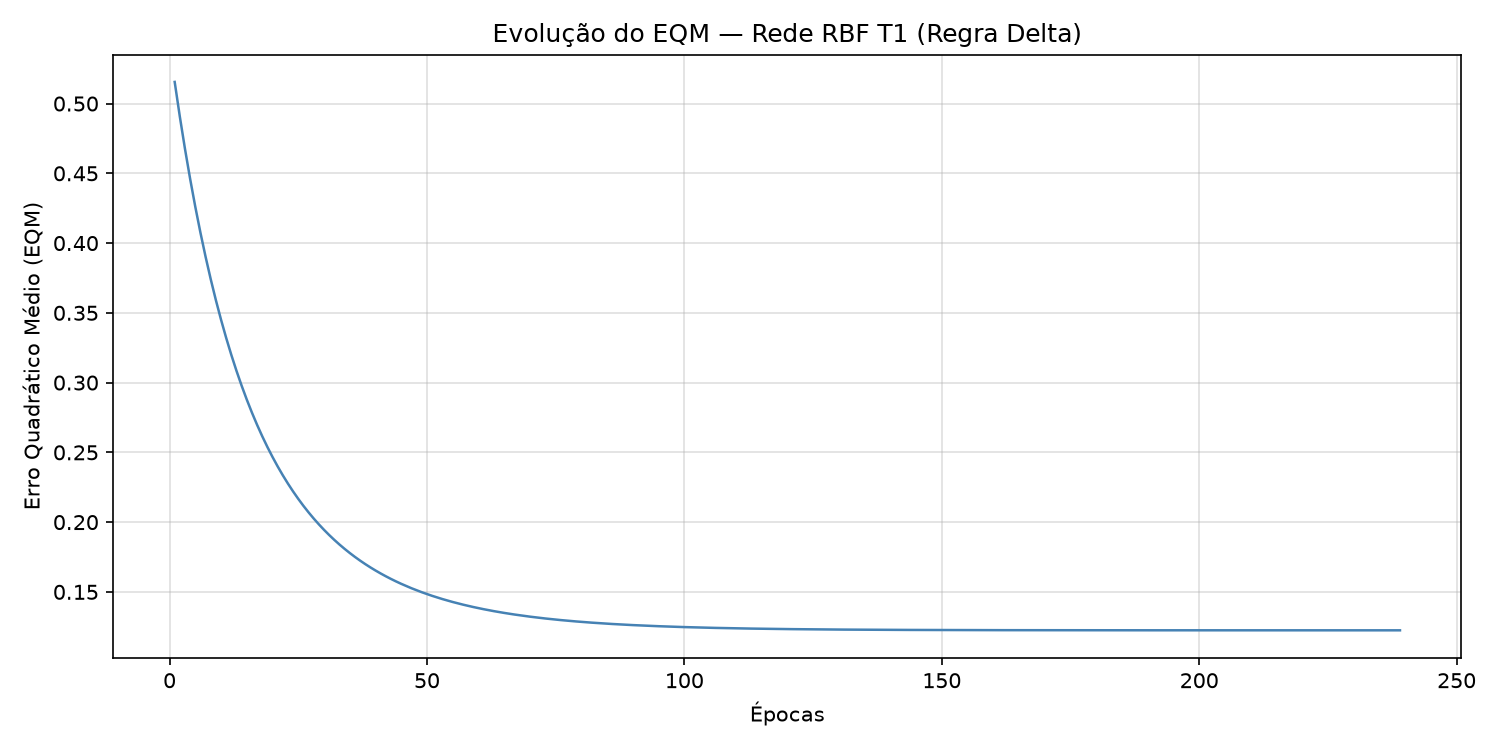
\includegraphics[width=1.23\textwidth]{../graphics/Evolucao_do_erro/treinamento_rbf_1.png}
    }
    \caption{Evolução do EQM em função do número de épocas no 1\textsuperscript{o} treinamento (T1).}
    \label{fig:eqm_t1}
\end{figure}

\begin{figure}[H]
    \centering
    \makebox[\textwidth][c]{%
        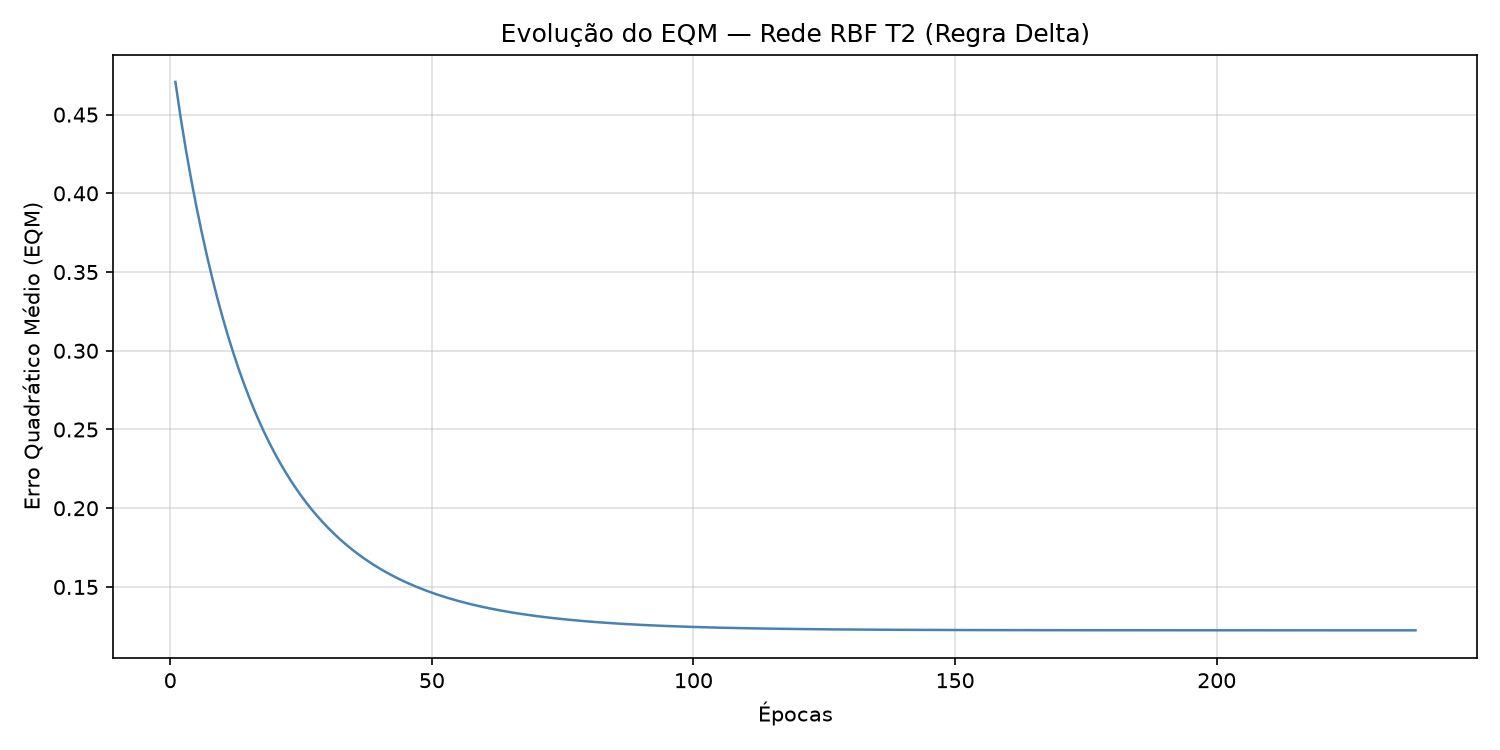
\includegraphics[width=1.23\textwidth]{../graphics/Evolucao_do_erro/treinamento_rbf_2.png}
    }
    \caption{Evolução do EQM em função do número de épocas no 2\textsuperscript{o} treinamento (T2).}
    \label{fig:eqm_t2}
\end{figure}

\begin{figure}[H]
    \centering
    \makebox[\textwidth][c]{%
        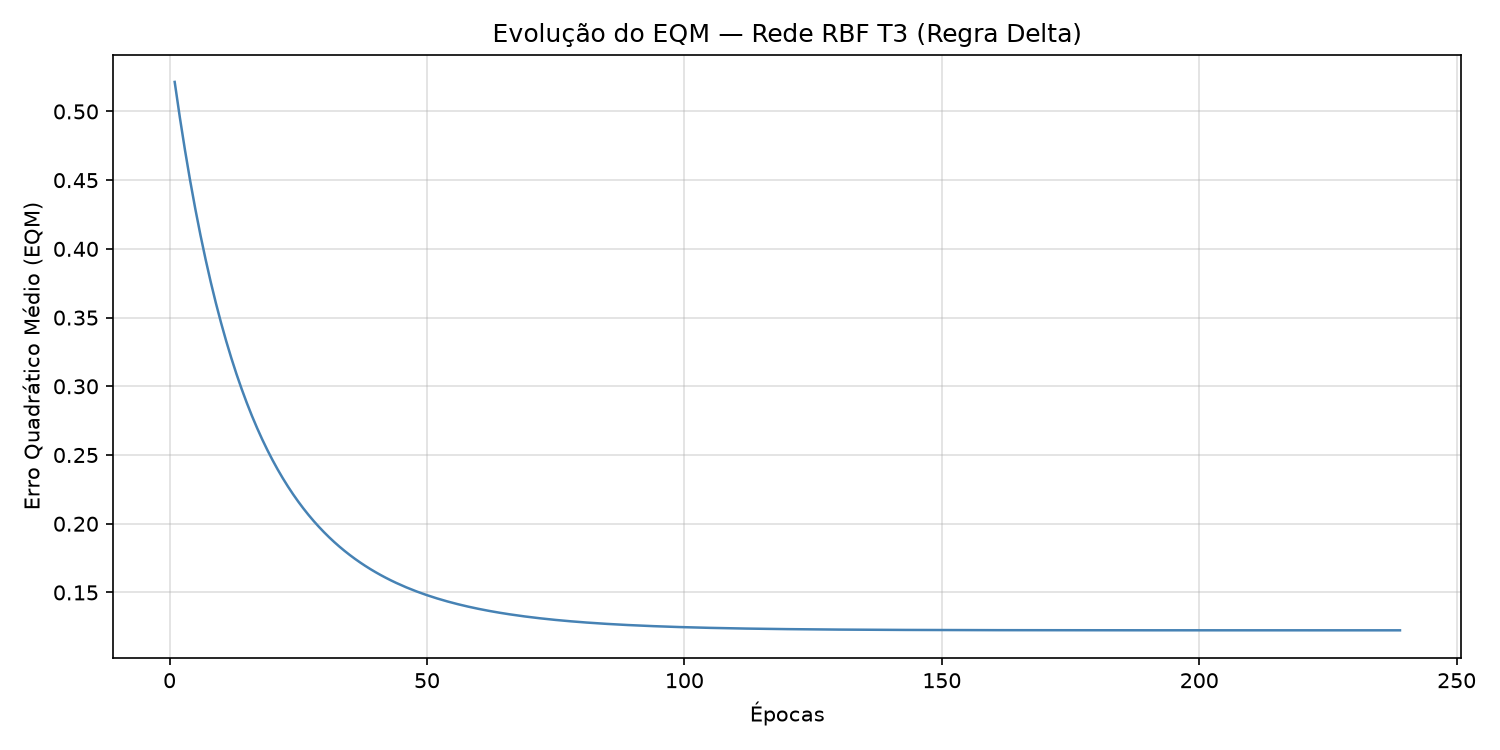
\includegraphics[width=1.23\textwidth]{../graphics/Evolucao_do_erro/treinamento_rbf_3.png}
    }
    \caption{Evolução do EQM em função do número de épocas no 3\textsuperscript{o} treinamento (T3).}
    \label{fig:eqm_t3}
\end{figure}

\begin{figure}[H]
    \centering
    \makebox[\textwidth][c]{%
        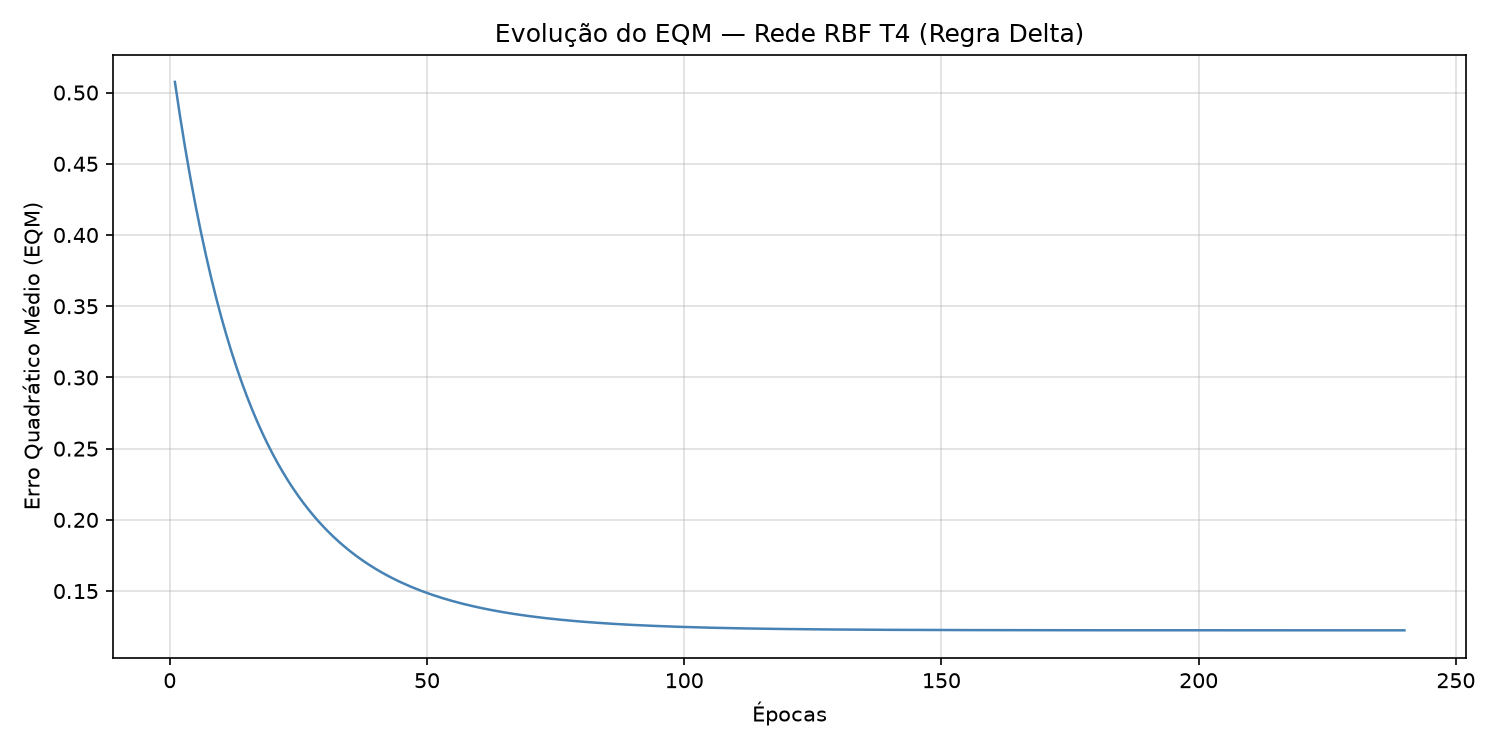
\includegraphics[width=1.23\textwidth]{../graphics/Evolucao_do_erro/treinamento_rbf_4.png}
    }
    \caption{Evolução do EQM em função do número de épocas no 4\textsuperscript{o} treinamento (T4).}
    \label{fig:eqm_t4}
\end{figure}

\begin{figure}[H]
    \centering
    \makebox[\textwidth][c]{%
        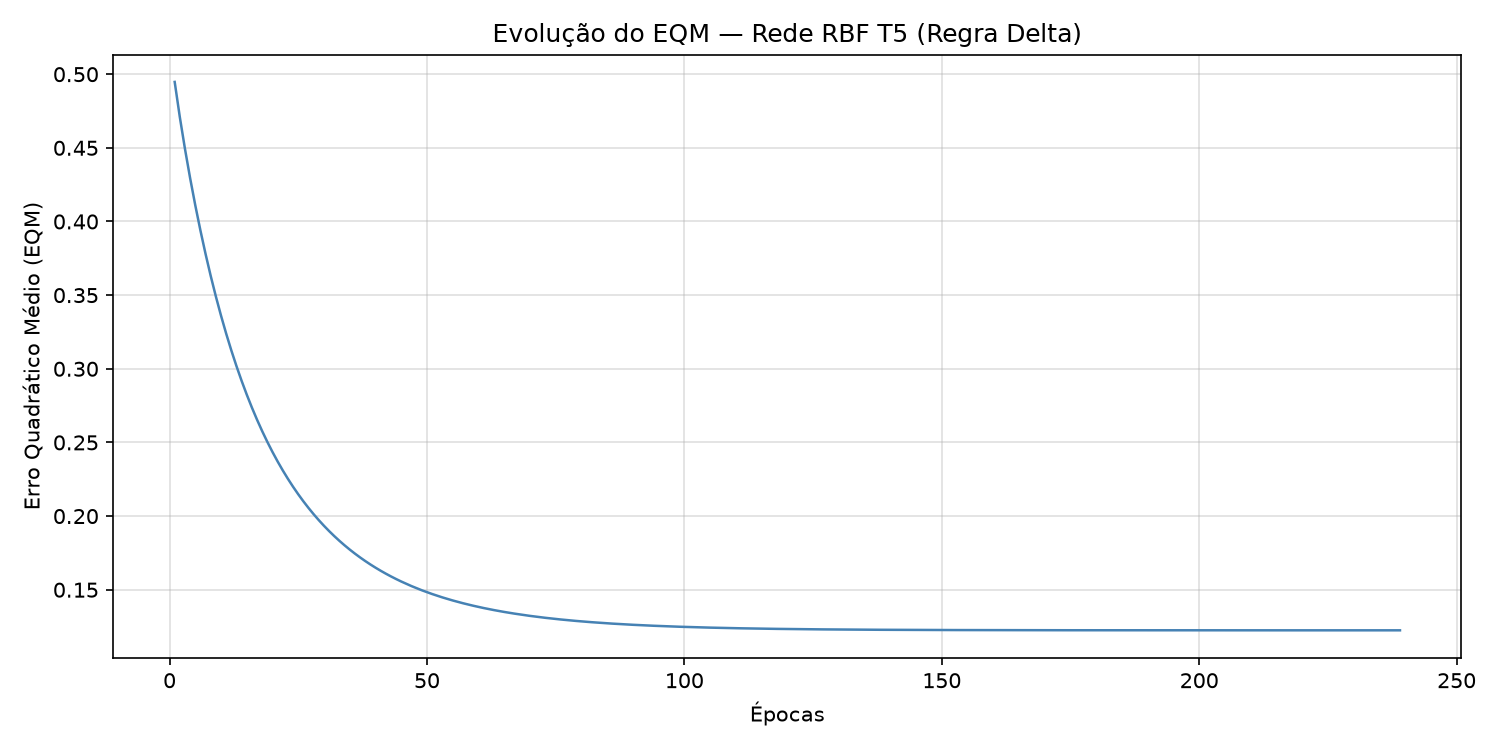
\includegraphics[width=1.23\textwidth]{../graphics/Evolucao_do_erro/treinamento_rbf_5.png}
    }
    \caption{Evolução do EQM em função do número de épocas no 5\textsuperscript{o} treinamento (T5).}
    \label{fig:eqm_t5}
\end{figure}

% =============================================================
\section*{5. Validação}
% =============================================================

A Tabela~\ref{tab:validacao} apresenta os resultados da validação com os dados de teste, aplicando o pós-processamento $y^{\text{pos}} = +1$ se $y \geq 0$ e $y^{\text{pos}} = -1$ se $y < 0$. Os resultados foram idênticos nos cinco treinamentos; os valores de $y$ exibidos correspondem ao treinamento T1.

\begin{table}[H]
    \centering
    \caption{Resultados da validação da rede RBF (Tabela 3 do roteiro – treinamento T1).}
    \label{tab:validacao}
    \renewcommand{\arraystretch}{1.3}
    \begin{tabular}{|c|c|c|c|c|c|}
        \hline
        \textbf{Amostra} & \textbf{$x_1$} & \textbf{$x_2$} & \textbf{$d$} & \textbf{$y$} & \textbf{$y^{\text{pos}}$} \\
        \hline
        1  & 0,8705 & 0,9329 & $-1$ & $-1{,}2733$ & $-1$ \\
        \hline
        2  & 0,0388 & 0,2703 & $+1$ & $+0{,}2209$ & $+1$ \\
        \hline
        3  & 0,8236 & 0,4458 & $-1$ & $-0{,}8110$ & $-1$ \\
        \hline
        4  & 0,7075 & 0,1502 & $+1$ & $+0{,}0753$ & $+1$ \\
        \hline
        5  & 0,9587 & 0,8663 & $-1$ & $-1{,}2783$ & $-1$ \\
        \hline
        6  & 0,6115 & 0,9365 & $-1$ & $-1{,}1354$ & $-1$ \\
        \hline
        7  & 0,3534 & 0,3646 & $+1$ & $+1{,}2813$ & $+1$ \\
        \hline
        8  & 0,3268 & 0,2766 & $+1$ & $+1{,}4095$ & $+1$ \\
        \hline
        9  & 0,6129 & 0,4518 & $-1$ & $+0{,}0012$ & $+1$ \\
        \hline
        10 & 0,9948 & 0,4962 & $-1$ & $-1{,}1730$ & $-1$ \\
        \hline
        \multicolumn{5}{|c|}{\textbf{Taxa de acertos}} & \textbf{90\%} \\
        \hline
    \end{tabular}
\end{table}

% =============================================================
\section*{6. Matriz de confusão e métricas}
% =============================================================

As Figuras~\ref{fig:conf_t1} a~\ref{fig:conf_t5} apresentam as matrizes de confusão obtidas nos cinco treinamentos. Em todos os casos, os resultados foram idênticos. A Tabela~\ref{tab:metricas} consolida as métricas de desempenho.

\begin{figure}[H]
    \centering
    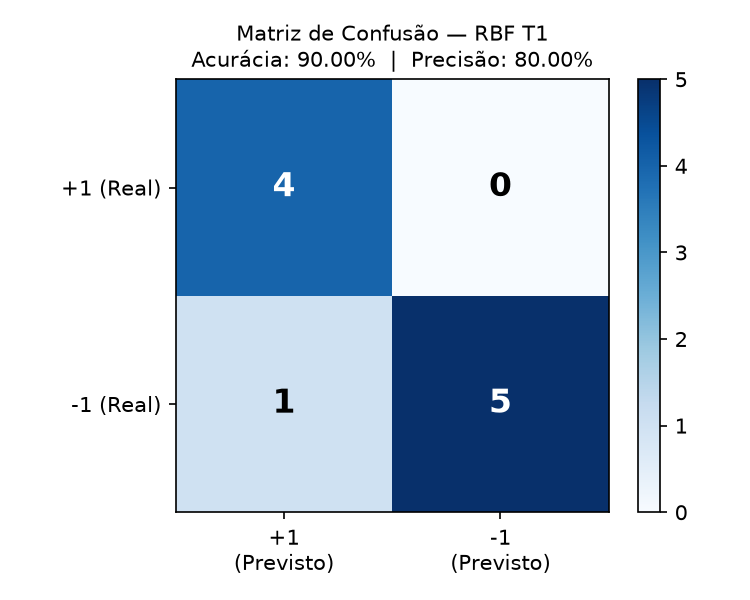
\includegraphics[width=0.55\textwidth]{../graphics/matrizes_de_confusao/rede_rbf_T1.png}
    \caption{Matriz de confusão – treinamento T1.}
    \label{fig:conf_t1}
\end{figure}

\begin{figure}[H]
    \centering
    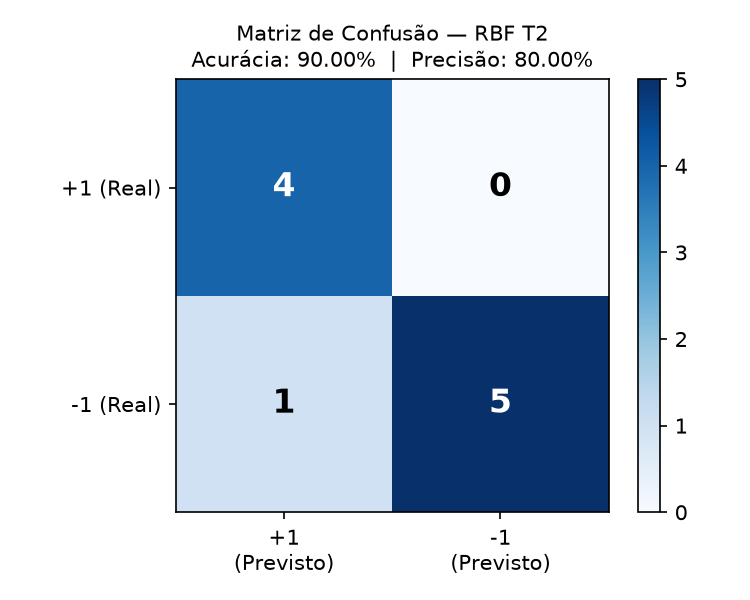
\includegraphics[width=0.55\textwidth]{../graphics/matrizes_de_confusao/rede_rbf_T2.png}
    \caption{Matriz de confusão – treinamento T2.}
    \label{fig:conf_t2}
\end{figure}

\begin{figure}[H]
    \centering
    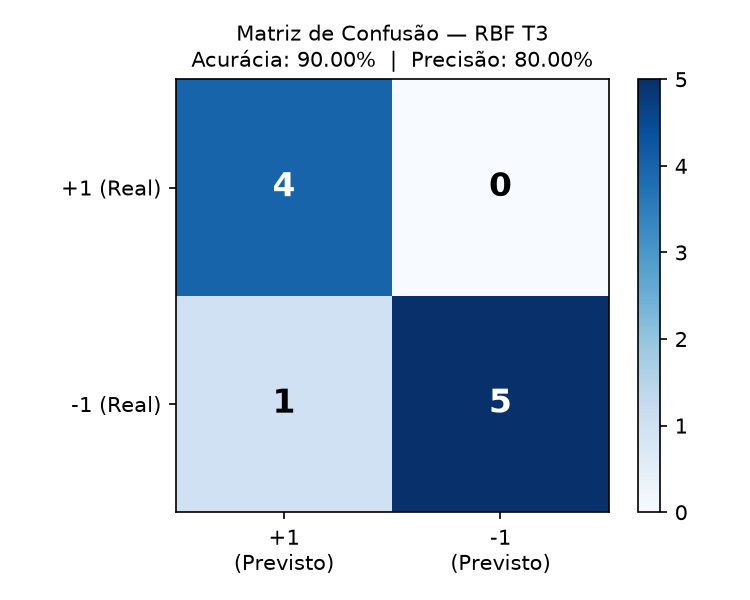
\includegraphics[width=0.55\textwidth]{../graphics/matrizes_de_confusao/rede_rbf_T3.png}
    \caption{Matriz de confusão – treinamento T3.}
    \label{fig:conf_t3}
\end{figure}

\begin{figure}[H]
    \centering
    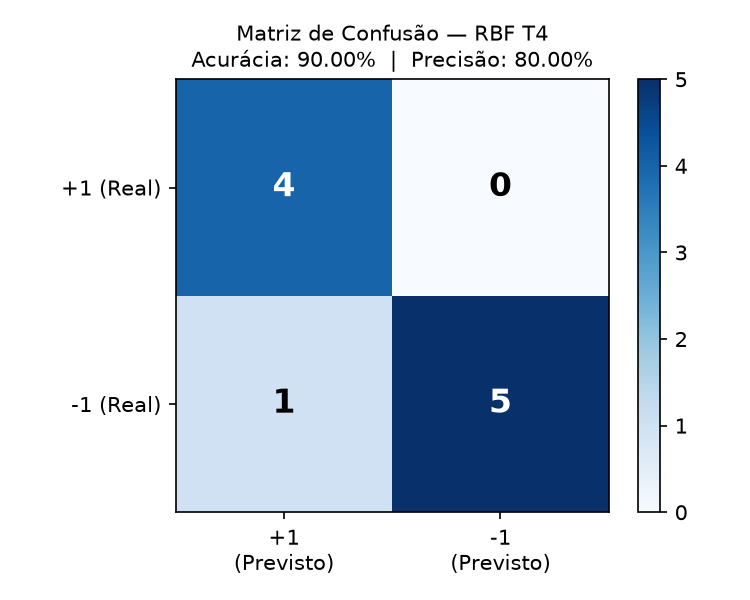
\includegraphics[width=0.55\textwidth]{../graphics/matrizes_de_confusao/rede_rbf_T4.png}
    \caption{Matriz de confusão – treinamento T4.}
    \label{fig:conf_t4}
\end{figure}

\begin{figure}[H]
    \centering
    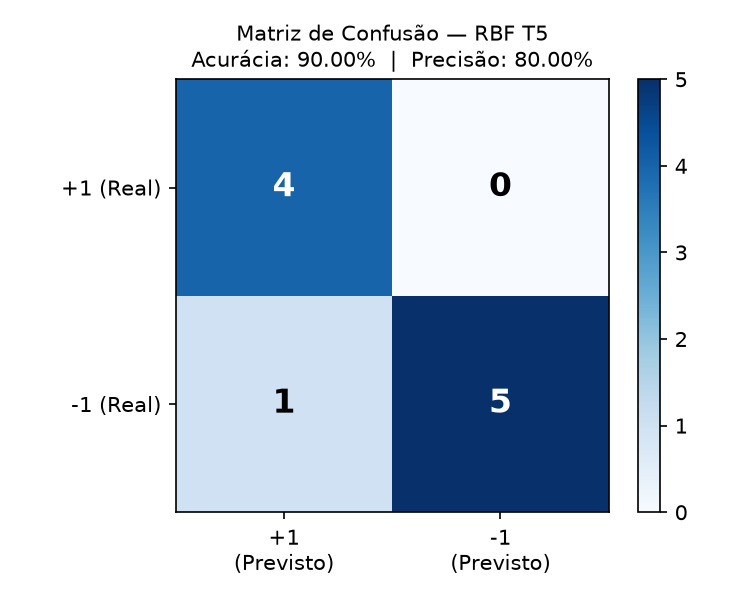
\includegraphics[width=0.55\textwidth]{../graphics/matrizes_de_confusao/rede_rbf_T5.png}
    \caption{Matriz de confusão – treinamento T5.}
    \label{fig:conf_t5}
\end{figure}

\begin{table}[H]
    \centering
    \caption{Métricas de desempenho da rede RBF na validação (resultados idênticos nos cinco treinamentos).}
    \label{tab:metricas}
    \renewcommand{\arraystretch}{1.3}
    \begin{tabular}{|l|c|}
        \hline
        \textbf{Métrica} & \textbf{Valor} \\
        \hline
        VP (Verdadeiro Positivo) & 4 \\
        \hline
        VN (Verdadeiro Negativo) & 5 \\
        \hline
        FP (Falso Positivo) & 1 \\
        \hline
        FN (Falso Negativo) & 0 \\
        \hline
        $N_{\text{acertos}}$ & 9 \\
        \hline
        $N_{\text{erros}}$ & 1 \\
        \hline
        Acurácia & 90,00\% \\
        \hline
        Sensibilidade & 100,00\% \\
        \hline
        Especificidade & 83,33\% \\
        \hline
        Precisão & 80,00\% \\
        \hline
    \end{tabular}
\end{table}

O único erro obtido é um Falso Positivo: a amostra 9 ($x_1 = 0{,}6129$, $x_2 = 0{,}4518$, $d = -1$) foi classificada como $+1$, com saída linear $y \approx +0{,}0012$ — valor marginalmente positivo. Essa amostra encontra-se em uma região limítrofe do espaço de entrada, com ativação gaussiana não negligenciável a partir do cluster 2 (centrado em $(0{,}399;\; 0{,}157)$). Estratégias para melhorar o desempenho incluem o aumento do número de clusters $K$ (mais neurônios na camada escondida) ou a ampliação do conjunto de treinamento, de forma a refinar a fronteira de decisão nessa região.

\end{document}
